\chapter{Motivación y antecedentes}
\label{ch:antecedentes}

%! Añadir lo de ultraembeddeed

%* Comprobar
Durante estas dos ultimas décadas, el bus USB (siglas en ingles de \emph{Universal Serial Bus} o Bus Serie Universal en castellano) se ha impuesto como uno de los grandes pilares de la comunicación en la informática moderna, no solo en productos de grandes masas (como dispositivos de almacenamiento o periféricos HID), sino también en sectores más complejos y robustos como lo son el militar o el industrial.

%* Comprobar
Al ser un bus tan ampliamente utilizado, existen multitud de ocasiones en las que sería de gran interés poder conocer que datos circula por él, ya sea para fines de seguridad\cite{NISSIM2017675}, control, ingeniería inversa o búsqueda y solución de problemas. Por ello, es de gran interés disponer de sistemas capaces de realizar dicha tarea de forma económica y sencilla.

%* Comprobar [mover posiblemente a apartado introducción]
A la hora de realizar la captura USB, existen dos técnicas diferentes, cada una con ciertas ventajas e inconvenientes, comentadas a continuación.
\begin{enumerate}
    \item \textbf{Por medio de un \textit{software} de captura en uno de los equipos implicados (Fig. ~\ref{fig:captura-SW}).} \\
    Método más sencillo, ya que no es necesario utilizar herramientas externas a parte del propio \textit{software}, pero con ausencia de varios datos de interés, como pueden ser el estado del Bus o los identificares de paquetes (PIDs).
    
    Posee a su vez limitaciones en su ejecución, ya que es necesario un completo acceso al equipo donde se realice la captura, existiendo además la posibilidad de no disponer de \textit{software} compatible para el mismo. 
    \begin{figure}[hbtp]
        \centering
        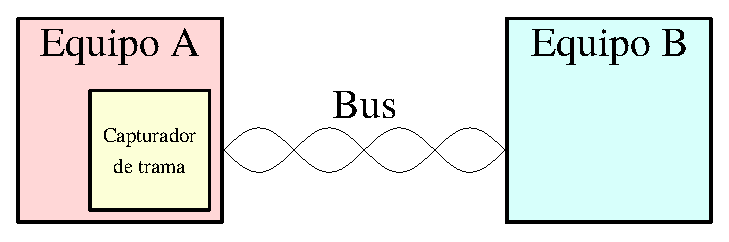
\includegraphics[scale=0.6]{esquemas/esquema-captura-software.eps}
        \caption{Esquema de captura por medio de \textit{software}}
        \label{fig:captura-SW}
    \end{figure}
    
    \item \textbf{Utilizando un elemento \textit{hardware} intermedio entre los equipos (Fig. ~\ref{fig:captura-HW}).} \\
    Método que permite un mayor control y compatibilidad al ser totalmente independiente a los equipos implicados, pero que debido al uso de herramientas externas y a la necesidad de utilizar un equipo extra donde grabar y procesar los datos obtenidos, hace que sea un método mas laborioso, y por lo general, mas costoso.
    Se obtiene una mayor cantidad de información comparado al método \textit{software} al tener un acceso directo al propio bus.
    \begin{figure}[hbtp]
        \centering
        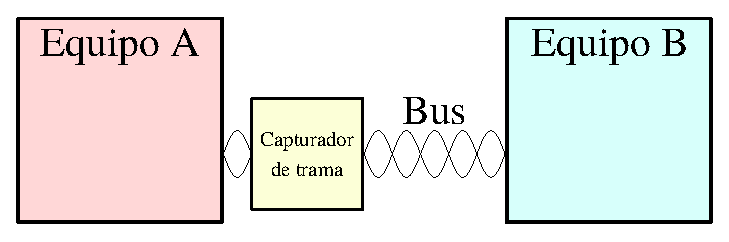
\includegraphics[scale=0.6]{esquemas/esquema-captura-hardware.eps}
        \caption{Esquema de captura por medio de \textit{hardware}}
        \label{fig:captura-HW}
    \end{figure}
\end{enumerate}

%! Revisar
\section{Sistemas \emph{software} actuales}
%* Comprobar
Debido a la gran facilidad y bajo coste que trae consigo el utilizar sistemas de captación \emph{software}, no es de extrañar que la gran mayoría de productos ya existentes se encuentran dentro de este grupo.

A continuación se muestra una lista detallada de los sistemas de captación \emph{Software} más relevantes, clasificados según su tipo de licencia y ordenados según la fecha de última actualización.

\subsection{Licencia de tipo \emph{shareware}\cite{hui2008economics}}
Es \emph{software} no gratuito, de código cerrado y libre distribución entre usuarios, que por lo general, posee un periodo de prueba en el que disfrutar la mayoría de las funciones sin coste. Todos las aplicaciones descritas a continuación poseen una interfaz gráfica e intuitiva, y funcionan unicamente bajo al Sistema Operativo \emph{Windows\texttrademark}.

\begin{itemize}
    %* Comprobar
    \item \textbf{\emph{USB Monitor}\footnote{Página web del producto: \url{https://www.hhdsoftware.com/usb-monitor}} de \emph{HHD Software Ltd}.} \\
    % De forma gráfica e intuitiva, este \emph{Software} monitoriza y analiza el tráfico USB existente en cualquier puerto de una máquina que funcione gracias al Sistema Operativo \emph{Windows\texttrademark}.
    Posee un periodo de prueba de 14 días en el que se permite utilizar todas las funciones sin restricciones.

    Cabe destacar que este sistema tiene cuatro ediciones\footnote{Comparación completa de las ediciones de pago: \url{https://www.hhdsoftware.com/usb-monitor/compare}}, comentadas a continuación.
    \begin{enumerate}
        \item \textbf{Edición \emph{standard}.} Es la versión más básica. Incluye las siguientes funciones:
        \begin{itemize}
            \item Soporte para todas las versiones de USB.
            \item Funciones básicas de monitorización y visualizado.
            \item Filtros básicos.
            \item Guardado básico.
            \item Estadísticas.
            \item Monitorización remota.
        \end{itemize}
        Su precio, a 27 de Marzo de 2019, es de 54.99\texteuro para uso NO comercial y 74.99\texteuro para uso comercial.

        \item \textbf{Edición gratuita\footnote{Se distribuye bajo el nombre de \emph{Free USB Analyzer} en: \url{https://freeusbanalyzer.com/}}.}Permite las mismas funciones que la edición \emph{standard}, limitando uso máximo a cinco sesiones diarias, cada una de 10 minutos.
        
        \item \textbf{Edición \emph{professional}.} Incluye las ventajas de la edición \emph{standard}, añadiendo:
        \begin{itemize}
            \item Conversión de datos y visionado de datos HID, imagen o audio, entre otros.
            \item Filtros en la captura.
            \item Capacidad de exportar los datos capturados de forma avanzada.
        \end{itemize}
        Su precio, a 27 de Marzo de 2019, es de 119.99\texteuro para uso NO comercial y 169.99\texteuro para uso comercial.
        
        \item \textbf{Edición \emph{ultimate}.} Incluye las ventajas de la edición \emph{professional}, añadiendo:
        \begin{itemize}
            \item Visor de paquetes USB en bruto.
            \item Monitorización simultanea de varios dispositivos.
            \item Scripts personalizados usando el lenguaje \emph{TypeSpript}.
        \end{itemize}
        Su precio, a 27 de Marzo de 2019, es de 159.99\texteuro para uso NO comercial y 224.99\texteuro para uso comercial.
    \end{enumerate}
    
    %* Comprobar
    \item \textbf{\emph{USB Sniffer}\footnote{Página web del producto: \url{https://www.eltima.com/products/usb-sniffer/}} de \emph{Eltima Software}.} \\
    \emph{Software} con 14 días de prueba, cuya versión completa tiene un precio único de mercado, a 27 de Marzo de 2019, de \$69.95 (sin incluir comisiones de cambio de divisa e impuestos).
    
    Hay que destacar las siguientes características\footnote{Lista completa de funciones: \url{https://www.eltima.com/products/usb-port-monitor\#tableCheckList}}.

    \begin{itemize}
        \item Vista completa y detallada de los datos entrantes y salientes.
        \item Soporte para \emph{HUBs} USB.
        \item Control de la captura según los datos de entrada.
        \item Soporte para todas las versiones de USB.
        \item Guardado avanzado de la trama capturada.
        \item Capacidad de marcar datos en la interfaz.
        \item Monitorización simultanea de varios dispositivos.
    \end{itemize}
    
    %! Revisar
    \item \textbf{\emph{USBlyzer}\footnote{Página web del producto: \url{http://www.usblyzer.com/}}.} \\
    Posee un periodo de prueba de 33 días sin ninguna restricción.

    \noWord [terminar]

    \begin{itemize}
        \item Vista avanzada jerarquizada de todos los USB disponibles.
        \item Análisis de actividad del bus.
        \item Filtrado avanzado cuando se realizan búsquedas o capturas.
        \item Decodificación de una gran variedad de tipos de datos.
        \item Exportación avanzada.
    \end{itemize}
    
    
    %* Comprobar
    \item \textbf{\emph{USBTrace}\footnote{Página web del producto: \url{http://www.sysnucleus.com/}} de \emph{SysNucleus}.} \\
    Igual que todos los anteriores, este programa utiliza una interfaz en la que mostrar y analizar en tiempo real el tráfico de puerto.

    Su periodo de prueba tiene una duración de 15 días, limitando además la cantidad total de la captura a 256Kb por sesión.

    Entre otras\footnote{Lista de funciones completas: \url{http://www.sysnucleus.com/usbtrace_features.html}}, sus funciones más destacables son:
    \begin{itemize}
        \item Facilidad de uso y visualización.
        \item Variedad de filtros.
        \item Guardado avanzado.
        \item Permite análisis de los drivers utilizados por el equipo. 
        \item Captura en segundo plano.
        \item Decodificaciones personalizadas de los datos del bus.
    \end{itemize}

    Su precio unitario, a 27 de Marzo de 2019, asciende hasta \$125.00 (sin incluir comisiones de cambio de divisa e impuestos).
\end{itemize}

\noWord[Quito las fotos??]
\begin{figure}[htbp]
    \centering
    \subfigure[\emph{USB Monitor} - \emph{HHD Software Ltd}]{
        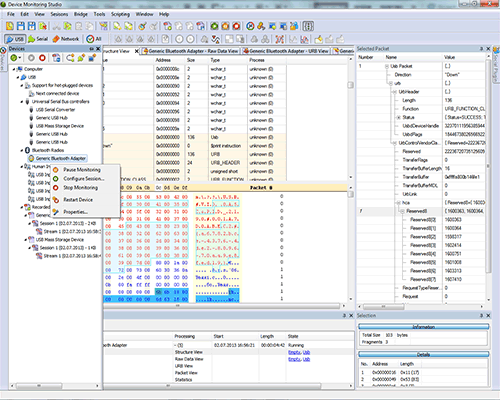
\includegraphics[width=60mm]{analizadores_software/HHD_Software-USB_Monitor.png}
        \label{fig:matriz-gui-close-sw:hdd}
    }
    \subfigure[\emph{USB Sniffer} - \emph{Eltima Software}]{
        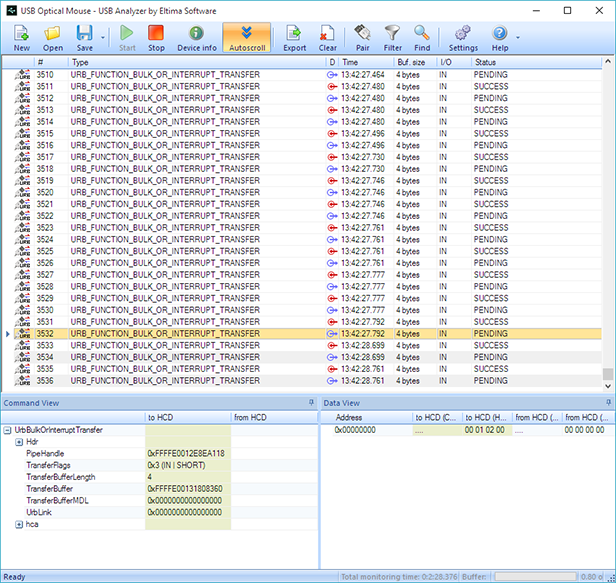
\includegraphics[width=60mm]{analizadores_software/eltima-USB_Sniffer.png}
        \label{fig:matriz-gui-close-sw:eltima}
    } \\
    \subfigure[\emph{USBlyzer}]{
        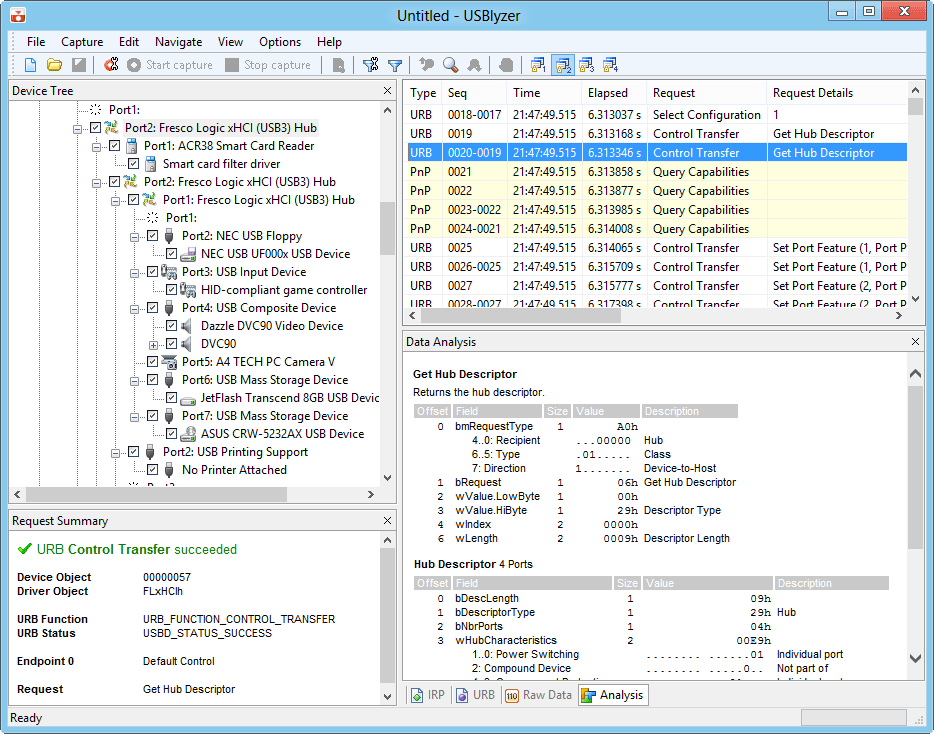
\includegraphics[width=60mm]{analizadores_software/usblyzer.png}
        \label{fig:matriz-gui-close-sw:usblyzer}
    }
    \subfigure[\emph{USBTrace} - \emph{SysNucleus}]{
        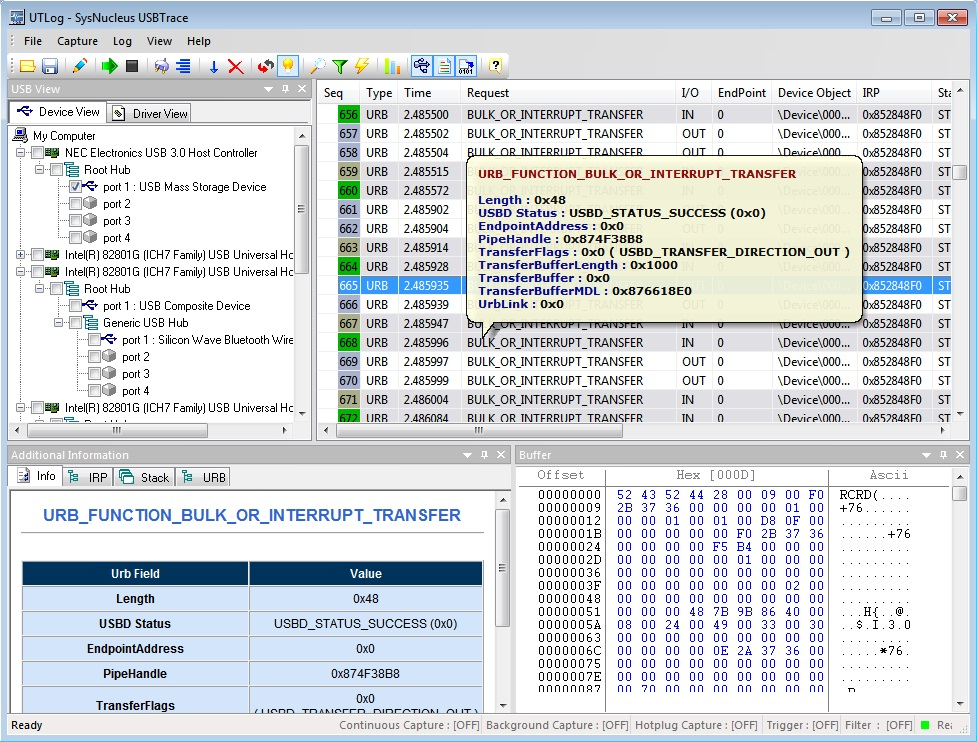
\includegraphics[width=60mm]{analizadores_software/SysNucleus-USBTrace.jpg}
        \label{fig:matriz-gui-close-sw:sysnucleus}
    }
    \caption{Interfaces gráficas de los analizadores \emph{software} de tipo \emph{shareware}. Imágenes extraídas de las páginas web de los desarrolladores.} 
    \label{fig:matriz-gui-close-sw}
\end{figure}


%* Comprobar
\subsection{Licencia de código libre\cite{gonzalez2003introduccion}}
Se trata de \emph{software} gratuito, cuyo código fuente está abiertamente disponible para su revisión y posibles modificaciones.

Dentro de este grupo hay que destacar dos herramientas, con funcionalidades similares, pero disponibles una bajo el Sistema Operativo \emph{Windows\texttrademark}, y la otra bajo sistemas \emph{UNIX-like}.

\begin{itemize}
    %* Comprobar
    \item \textbf{\emph{Tcpdump}\footnote{Página web del \emph{Software}: \url{https://www.tcpdump.org/}}.} \\
    Herramienta, que a través de una linea de comandos, es capaz de capturar, analizar y almacenar en un archivo PCAP paquetes de una amplia variedad de interfaces, entre las que se encuentra dispositivos \emph{USB}.

    Este método, debido a su especialización, no sería capaz de realizar un análisis detallado, por lo que sería necesario un programa adicional que posteriormente haga el estudio y clasificación de los datos de forma gráfica.

    Funciona en sistemas \emph{UNIX-like} (siempre que se tenga acceso la interfaz USB) bajo una licencia BSD\footnote{Información detallada de la licencia: \url{https://www.tcpdump.org/license.html}}.
    
    %* Comprobar
    \item \textbf{\emph{USBPcap}\footnote{Página web del \emph{Software}: \url{https://desowin.org/usbpcap/}}.}
    Realiza las mismas funciones que \emph{Tcpdump}, pero funcionando bajo el Sistema Operativo Windows con licencias GPLv2 y BSD.
    
    Sigue siendo necesario el uso de \emph{software} de terceros para su análisis completo.
\end{itemize}

%* Comprobar
Dichos archivos generados, por lo general de tipo \emph{pcap}\cite{guyharris2015}, se pueden analizar a través de la herramienta de análisis de paquetes \emph{Wireshark}\footnote{Página web del \emph{Software}: \url{https://www.wireshark.org/}}. Cabe destacar, que esta herramienta, y unicamente bajo sistemas basado en \emph{Linux}, puede ser capaz de capturar directamente y en tiempo real las tramas \emph{USB}. 

% \subsection{Licencia de código libre\cite{gonzalez2003introduccion}}
% Se trata de \emph{software} gratuito cuyo código fuente está disponible para su revisión y modificación.

% Principalmente hay que destacar dos herramientas, con funcionalidades similares, poro disponibles bajo dos 

% \begin{itemize}
%     \item \textbf{\emph{Tcpdump}\footnote{Página web del \emph{Software}: \url{https://www.tcpdump.org/}}.} \\
%     Herramienta, que a través de una linea de comandos, es capaz de capturar, analizar y almacenar en un archivo PCAP paquetes de una amplia variedad de interfaces, entre las que se encuentra dispositivos \emph{USB}.

%     Este método, debido a su especialización, no sería capaz de realizar un análisis detallado, por lo que sería necesario un programa adicional que posteriormente haga el estudio y clasificación de los datos de forma gráfica.

%     Funciona en sistemas \emph{UNIX-like} (siempre que se tenga acceso la interfaz USB) bajo una licencia BSD\footnote{Información detallada de la licencia: \url{https://www.tcpdump.org/license.html}}.
    
%     \item \textbf{\emph{USBPcap}\footnote{Página web del \emph{Software}: \url{https://desowin.org/usbpcap/}}.}
%     Realiza las mismas funciones que \emph{Tcpdump}, pero funcionando bajo el Sistema Operativo Windows con licencias GPLv2 y BSD.

%     Sigue siendo necesario el uso de \emph{software} de terceros para su análisis completo.
    
%     \item \textbf{\emph{Wireshark}\footnote{Página web del \emph{Software}: \url{https://www.wireshark.org/}}.}
%     Herramienta de análisis de paquetes, que de forma gráfica, es capaz de mostrar de forma ordenada sus diversas partes.

%     Los archivos de captura generados en los 

%     Bajo sistemas Linux, es
% \end{itemize}
    

%! Revisar
\section{Sistemas \emph{hardware} actuales}
En caso de que no sea posible la utilización de una captura por \emph{Software}, ya sea por incompatibilidades, falta de acceso, necesidad de obtener más datos de interés o cualquier otra causa, se tendría que utilizar un sistema más complejo, por medio de \emph{Hardware}.

%* Comprobar 
A continuación se muestran varios ejemplos ya existentes de este tipo, todos ellos soportan hasta la versión 2.0 de USB. \\

\textit{Nota. Todos los precios de la siguiente lista, excepto que se indique, no incluyen envío, impuestos locales, o tasas de cambio de divisa.}

\begin{itemize}
    %* Comprobar 
    \item \textbf{\emph{USB Explorer 200} de \emph{Ellisys}\footnote{Página web del producto: \url{https://www.ellisys.com/products/usbex200/index.php}}.}
    
    Sistema comercial, que entre otras características\cite{ellisys2008}, destacan:
    \begin{itemize}
        \item Soporte para USB 2.0 \emph{high speed} (480 Mbit/s), \emph{full speed} (12 Mbit/s) y \emph{low speed} (1.5 Mbit/s).
        \item \emph{Trigger} externo de hasta 5V de entrada o 3.3V de salida.
        \item Memoria interna FIFO de 32MBytes.
        \item Alimentación a través de la propia conexión USB en el equipo de análisis.
        \item Dimensiones aproximadas de 150x120x65mm con un peso de 750 gramos. Vease figura~\ref{fig:ellisys-Explorer200}.
    \end{itemize}

    Aun siendo el mismo producto, este está limitado por \emph{Software}, existiendo tres variaciones, cada una con más funcionalidades y mayor precio respecto a la anterior.

    \begin{enumerate}
        \item \textbf{Edición básica.}
        Es la versión más básica, permitiendo unicamente capturar y posteriormente almacenar en el equipo de análisis la trama USB. \\
        Su precio, a 27 de Marzo de 2019, es de 799\texteuro.
      
        \item \textbf{Edición estándar.}
        Incluye las ventajas de la edición básica, añadiendo:
        \begin{itemize}
            \item Captura en tiempo real.
            \item Filtros de captura.
            \item Resumen del tráfico existente.
            \item Decodificación parcial del protocolo USB.
        \end{itemize}
        Su precio, a 27 de Marzo de 2019, es de 1599\texteuro.
        
        \item \textbf{Edición profesional.}
        Incluye las ventajas de la edición estándar, añadiendo:
        \begin{itemize}
            \item Decodificación completa USB.
            \item Análisis del protocolo.
            \item Capacidad de usar disparos (\emph{triggers}) externos.
        \end{itemize}
        Su precio, a 27 de Marzo de 2019, es de 3199\texteuro.
    \end{enumerate}    
    \begin{figure}[htb]
        \centering
        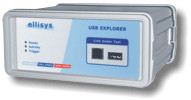
\includegraphics[width=50mm]{analizadores_hardware/ellisys_USBExplorer200.jpg}
        \caption{\emph{Ellisys USB Explorer 200}. Imagen extraída de la página web del fabricante.}
        \label{fig:ellisys-Explorer200}
    \end{figure}
    
    %* Comprobar
    \item \textbf{\emph{Mercury T2} de \emph{Teledyne LeCroy}\footnote{Página web del producto: \url{https://teledynelecroy.com/protocolanalyzer/usb/mercury-t2}}.}
    
    Sistema comercial, que entre otras características\cite{teledynelecroy2014}, destacan:
    \begin{itemize}
        \item Soporte para USB 2.0 \emph{high speed} (480 Mbit/s), \emph{full speed} (12 Mbit/s) y \emph{low speed} (1.5 Mbit/s).
        \item Memoria interna de 256MBytes.
        \item Captura automática en disco para permitir capturas de larga duración.
        \item \emph{Trigger} externo (necesario adaptador externo no incluido).
        \item Alimentación a través de la propia conexión USB en el equipo de análisis.
        \item Dimensiones aproximadas de 80x90x24mm con un peso de 158 gramos. Véase figura~\ref{fig:TeledyneLeCroy-MercuryT2}.
    \end{itemize}
    
    De igual manera que en el producto anterior, este posee varias versiones.

    \begin{enumerate}
        \item \textbf{Edición estándar.}
        Incluye las siguientes opciones:
        \begin{itemize}
            \item Captura y almacenaje de cualquier trama USB hasta 2.0 en tiempo real.
            \item Disparos (\emph{triggers}) para almacenar captura tanto externos, como detectando patrones en la trama.
        \end{itemize}
        Su precio, a 27 de Marzo de 2019, es de \$901.
        
        \item \textbf{Edición avanzada.}
        Incluye las ventajas de la edición estándar, añadiendo:
        \begin{itemize}
            \item Estadísticas en tiempo real del bus.
            \item Exportación en formato .csv.
            \item API de automatización.
        \end{itemize}
        Su precio, a 27 de Marzo de 2019, es de \$1235.
    \end{enumerate}
    \begin{figure}[htb]
        \centering
        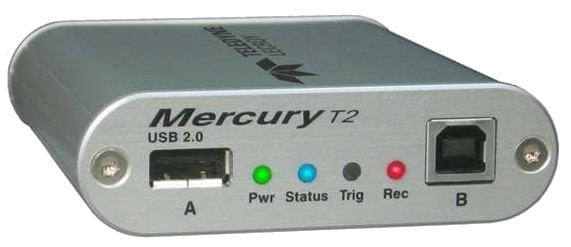
\includegraphics[width=50mm]{analizadores_hardware/TeledyneLeCroy_MercuryT2.jpg}
        \caption{\emph{Teledyne LeCroy Mercury T2}. Imagen extraída de la página web del fabricante.}
        \label{fig:TeledyneLeCroy-MercuryT2}
    \end{figure}

    %* Comprobar
    \item \textbf{\emph{Beagle USB} de \emph{Total Phase}\footnote{Página web del producto: \url{https://www.totalphase.com/protocols/usb/}}.}
    
    Dentro de la amplia gama de productos que disponen, hay dos que destacan principalmente.
    \begin{enumerate}
        \item \textbf{\emph{Beagle USB 480}\cite{totalphase12-2018}.}
        De todas las versiones que poseen, esta es la más básica que permite hasta capturas \emph{high speed} de (480 Mbit/s).
        \begin{itemize}
            \item Captura en tiempo real.
            \item Estadísticas en tiempo real.
            \item 64MBytes de memoria integrada.
            \item \emph{Triggers} externos de entrada y salida.
            \item Sincronización básica.
            \item API de control.
        \end{itemize}
        Su precio, a 27 de Marzo de 2019, es de \$2250.
        
        \item \textbf{\emph{Beagle USB 480 Power}\cite{totalphase480-2018} - Edición estándar.}
        Posee las mismas ventajas que el producto anterior, pero aumentando la memoria integrada de 64MBytes a 256MBytes y añadiendo capacidad de medir la tensión y corriente del propio Bus.\\
        Su precio, a 27 de Marzo de 2019, es de \$1599.
        
        \item \textbf{\emph{Beagle USB 480 Power}\cite{totalphase480-2018} - Edición \emph{ultimate}.}
        Mejora las capacidades de disparos (\emph{triggers}) respecto a la versión estándar.\\
        Su precio, a 27 de Marzo de 2019, es de \$2950.
    \end{enumerate}
    
    \begin{figure}[htbp]
        \centering
        \subfigure[\emph{Beagle USB 480}]
        {
            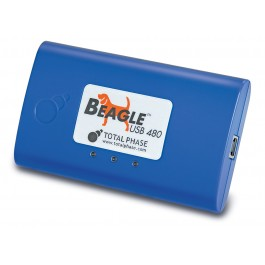
\includegraphics[width=40mm]{analizadores_hardware/TotalPhase_beagle480.jpg}
            \label{fig:TotalPhase-480}
            }
            \subfigure[\emph{Beagle USB 480 Power}]{
                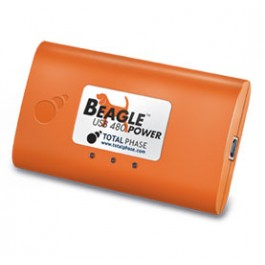
\includegraphics[width=40mm]{analizadores_hardware/TotalPhase_beagle480Power.jpg}
                \label{fig:TotalPhase-480Power}
                }
                \caption{Productos de \emph{Total Phase}. Imágenes extraídas de la página web del fabricante.} 
                \label{fig:TotalPhase}
            \end{figure}
    
    %!
    \item \textbf{USB Sniffer - UltraEmbedded}
\end{itemize}

\section{Comparación de sistemas / Tabla resumen}


\begin{table}[hbtp]
    \centering
    \begin{tabular}{|c|c|c|c|c|}
        \hline
        Nombre & Licencia & Precio & Ventajas & Inconvenientes \\ \hline
        \hline

        \emph{USB Monitor} &
        \emph{Shareware} &
        Desde 54.99\texteuro &
        d &
        i \\ \hline

        \emph{USB Sniffer} &
        \emph{Shareware} &
        Desde \$69.95 &
        d &
        i \\ \hline

        \emph{USBlyzer} &
        \emph{Shareware} &
        Desde \$108 &
        d &
        i \\ \hline

        \emph{USBTrace} &
        \emph{Shareware} &
        Desde \$125 &
        d &
        i \\ \hline

        \emph{\begin{tabular}{@{}c@{}}Tcpdump /\\ USBPcap\end{tabular}} &
        \emph{Código libre} &
        -- &
        d &
        i \\ \hline
    \end{tabular}
    \caption{Tabla comparativa de sistemas \emph{software}}
    \label{tabla:comparativa-sw}
\end{table}

% \chapter{Motivación y antecedentes}
% \label{ch:antecedentes_plantilla}

% El problema que pretendes resolver está dentro de un contexto que el cliente debe conocer.  Esta sección aporta información para conocer en detalle la importancia del problema y la dificultad para resolverlo con los productos y programas disponibles actualmente.

% Este capítulo concentrará el grueso de las citas del TFG.  Dado que se trata del primer trabajo profesional, el alumno no suele estar familiarizado con las citas bibliográficas.  Pon toda tu atención en qué citas y cómo lo citas.  Revisa la sección~\ref{sec:bibliografia-citas} para las reglas mínimas que deben cumplir las citas.

% \warning{Es muy importante respetar la regla de atribuir correctamente.  No es aceptable desde el punto de vista legal, ni tampoco desde el punto de vista ético, copiar trabajo de otros sin atribuirlo correctamente a los autores.}

% Esta sección debe estudiar de forma sistemática todas las opciones ya disponibles en la actualidad para resolver el problema. No basta con una mera enumeración, hay que estudiarlos mínimamente para explicar por qué no son una solución para el problema o qué podría aportar a la solución del problema.

% Un método sistemático para realizar esta parte del TFG es la revisión sistemática de literatura, conocida habitualmente por sus siglas en inglés SLR (\emph{Sistematic Literature Review}).  Un resumen muy sencillo de cómo realizar una SLR puede encontrarse en~\cite{anderskofodpetersen2014}.  También encontrarás consejos prácticos en~\cite{sandroschulze2017}.  Para un proceso más detallado, especialmente si tu problema tiene mucho arte previo, puedes consultar~\cite{barbarakitchenhamstuartcharters2007}.  Si no hay mucho arte previo pon este capítulo y el siguiente juntos.

% En una tesis doctoral el análisis sistemático del estado del arte es esencial. En un TFG es importante, pero no hay que perder la cabeza.  Un TFG son unas 300 horas de trabajo de un estudiante medio que ya posea los conocimientos generales necesarios (volveremos a esto más tarde).  Considero que un buen análisis del estado del arte corresponde a un trabajo de entre 25 horas y 100 horas, dependiendo del tema del proyecto.  Si el tema es muy específico es más fácil hacer el estudio del estado del arte.

% Termina este capítulo con una sección que resuma el estado del arte e identifique las lagunas lo más claramente posible.  Una tabla comparativa o un gráfico pueden ser formas interesantes de presentar la información.